

\clearpage
\chapter{Recursive descent parser}

\section{Aim}
To design and construct a recursive descent parser for the given expression.
\begin{algorithmic}[1]
	\State $E\: \quad \rightarrow$ $T \; E’$
	\State $E’  \quad \rightarrow$ $+ \; T \; E’ \; | \; e$
	\State $T\: \quad \rightarrow$ $F \; T’$
	\State $T’  \quad \rightarrow$ $* \; F \; T’ \; | \; e$
	\State $F\: \quad \rightarrow$ $( \; E \; ) \; | \; id$
\end{algorithmic}




\section{Theory}
Top-down parsing can be viewed as the problem of constructing a parse tree for the input string, starting from the root and creating the nodes of the parse tree in pre-order. Equivalently, top-down parsing can be viewed as finding a leftmost derivation for an input string. At each step of a top-down parse, the key problem is that of determining
the production to be applied for a non-terminal. Once an production is chosen, the rest of the parsing process consists of "\textit{matching}" the terminal symbols in the production body with the input string.


Recursive descent parser is a general form of top-down parsing, which may require backtracking to find the correct production to be applied. On the other hand, a special case of recursive-descent parsing where no backtracking is required is call predictive parsing. Predictive parsing chooses the correct production by looking ahead at the input a fixed number
of symbols.

A recursive-descent parsing program consists of a set of procedures, one for each
non-terminal. Execution begins with the procedure for the start symbol, which halts and announces success if its procedure body scans the entire input string.
General recursive-descent may require backtracking; that is, it may require
repeated scans over the input.

\section{Algorithm}

\begin{algorithm}[H]
	\caption{Non-predictive recursive descent parser without backtracking}
	\begin{algorithmic}[1]
		\Procedure{A}{ }\Comment{A : Non-terminal of grammar}
			
			\State Choose an A-production, $A \gets X X . . . X_k$
					
			\For{$ i = 1$ to $k$}
				\If{$X_i$ is a nonterminal}
					\State Call procedure \Call{$X_i$}{ }
				\ElsIf{$X_i$ equals to the current input symbol $a$}
					\State Advance the input to the next symbol
				\Else
					\State Error Occurred
				\EndIf
			\EndFor
		\EndProcedure
		\State \Call{StartSymbol}{ } \Comment{Call start symbol to
		 start parsing}		
	\end{algorithmic}
\end{algorithm}

\begin{algorithm}[H]
	\caption{Non-predictive recursive descent parser with backtracking}
	\begin{algorithmic}[1]
		\Procedure{A}{ }\Comment{A : Non-terminal of grammar}
		
			\State $inputState \gets CurrentInputState$ 
			\ForAll{production $P=X X . . . X_k \in A-productions$}
				\State $backtrack =$ FALSE
				\For{$ i = 1$ to $k$}
					\If{$X_i$ is a nonterminal}
						\State Call procedure \Call{$X_i$}{ }
					\ElsIf{$X_i$ equals to the current input symbol $a$}
						\State Advance the input to the next symbol
					\Else \Comment{Error occurred, iterate to next production}
						\State $backtrack = TRUE$ 
						\State $break$
					\EndIf
				\EndFor
				\If{$bracktrack = TRUE$}
					\State $input \gets inputState$ \Comment{Restore input status}
				\Else \Comment{Completely parsed a production}
					\State $break$
				\EndIf
			\EndFor
		\EndProcedure
		\State \Call{StartSymbol}{ } \Comment{Call start symbol to start parsing}		
	\end{algorithmic}
\end{algorithm}

\begin{figure}[!h]
	\centering
	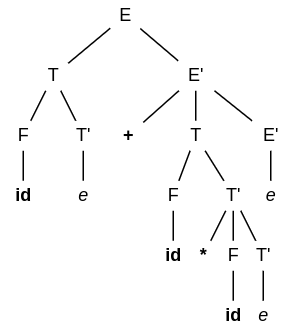
\includegraphics[height=3in]{../EXP6/diagram.png}
	\caption{Top down parser for id+id*id}
\end{figure}

\break
\section{C-Program}
\lstinputlisting[style=CStyle,language=C]{../EXP6/recursive_descent.c}

\section{Output}
\textbf{Output1}
\lstinputlisting[style=plain]{../EXP6/output1.txt}
\textbf{Output2}
\lstinputlisting[style=plain]{../EXP6/output2.txt}

\section{Result}
The program compiled and successfully parsed an given expression via non predictive recursive descent with backtracking.